\subsection{Banco de pruebas}
\subsubsection{Elementos}
Se decidió que el banco de pruebas cuente con los siguientes elementos:
\begin{itemize}
	\item interruptor
	\item botón de marcha/ parada
	\item botón parada de emergencia
	\item señalización lumínica
	\item freno para generar perturbaciones 
	\item riel para colocar un nuevo motor que actuará como carga
	\item Panel de control
		\subitem Botón de emergencia
		\subitem Encendido/ apagado
		\subitem Potenciómetro para variar velocidad
		\subitem Display para observar velocidad
		\subitem Alarmas visuales
\end{itemize}
\subsubsection{Presupuesto--Valor--Costo a tal día}
\subsection{HMI}

Se realizó una interfaz humana maquina con los siguientes elementos:
	\begin{itemize}
		\item boton de start(acá o en el tablero???)
		\item varias velocidades configuradas previamente
		\item inversión y señalización del mismo
		\item torque???
		\item HMI
        	\subitem Alarmas
       		\subitem Información en tiempo real
        	\subitem Histórico de datos
        	\subitem Control general del banco
	\end{itemize}
	\begin{figure}[htb]
		\centering
		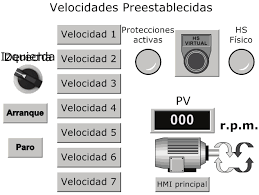
\includegraphics{HMIej.png}
		%\caption{Placa BME280}
		%\label{fig:BME280}
	\end{figure}

\newpage